%!TEX root = Economics and Behaviour.tex


\chapter{Standard theoretic basics for analysis of strategic behaviour}


\section{Games in strategic form}
To display a static game with two players ($P1$ and $P2$) and a finite number of possible signals (for simplicity lets assume that there are only two signals and call them $a$ and $b$) we usually use the matrix form where $u_{i}(x, y)$ represents the utility function for player $i$ given the signal $x$ for $P1$ and the signal $y$ for $P2$ with $x, y \in \{ a, b\}$.
\begin{center}
	\begin{tabular}{|c|c|c|}
		\hline\hline
  			$P1$ / $P2$ & \textbf{a} & \textbf{b} \\
         		\cline{1-3}
   					\textbf{a} & $( u_{1}(a, a) , u_{2}(a, a))$ & $(u_{1}(a, b), u_{2}(a, b))$	\arrayrulewidth2pt \\
            	\cline{1-3}
   					\textbf{b} & $( u_{1}(b, a), u_{2}(b, a))$ & $(u_{1}(b, b), u_{2}(b, b))$\\ \hline\hline
	\end{tabular}	
\end{center}

We call a \begriff{set of strategies} a complete plan of actions for each situation in a game.

\begin{example}[Prisoner's Dilemma] \label{prisonersdilemma} \index{Prisoner's Dilemma}
	 Image, two members of a criminal gang are arrested and imprisoned. Each prisoner is in solitary confinement with no means of communicating with the other. The prosecutors lack sufficient evidence to convict the pair on the principal charge. They hope to get both sentenced to a year in prison on a lesser charge. Simultaneously, the prosecutors offer each prisoner a bargain. Each prisoner is given the opportunity either to: betray the other by testifying that the other committed the crime, or to cooperate with the other by remaining silent. The offer is:
	\begin{itemize}
		\item If A and B each betray the other, each of them serves 6 years in prison
		\item If A betrays B but B remains silent, A will be set free and B will serve 9 years in prison (and vice versa)
		\item If A and B both remain silent, both of them will only serve 1 year in prison (on the lesser charge)
	\end{itemize}
	
\begin{center}
	\begin{tabular}{|l|l|r|}
		\hline\hline
  			P1 / P2 & \textbf{defects} & \textbf{cooperates} \\
         		\cline{1-3}
   			\textbf{defects} & $(-6, -6)$ & $(0, -9)$ 	\arrayrulewidth2pt \\
            	\cline{1-3}
   			\textbf{cooperates} & $(-9, 0)$ & $(-1, -1)$ \\ \hline\hline
	\end{tabular}	
\end{center}


	Other Interpretations of the Prisoner's Dilemma
	\begin{itemize}
		\item Collusion on prices
		\item Investing in human capital vs. arming for a war
		\item Buying a SUV vs. a smaller car
	\end{itemize}
\end{example}


\subsection{Dominant strategies}

\begin{definition}[Strict dominance] \index{strictly dominated}
	A strategy $s_{i}''$ is strictly dominated if and only if there exists another strategy $s_{i}'$ such that
	\[ u(s_{i}', s_{-i}) > u(s_{i}'', s_{-i}) \quad \forall s_{-i} \in S_{i} \]	
\end{definition}

In the \hyperref[prisonersdilemma]{Prisoner's Dilemma} $cooperate$ is strictly dominated by $defect$. Simply the elimination of strictly dominated strategies leads to the prediction of $(defects, defects)$, even though $(cooperates, cooperates)$ would result in a lower prison sentence.


\begin{example}
	Iterated elimination of strictly dominated strategies leads to
	\begin{itemize}
		\item for Player 2: $l$ strictly dominates $r$
		\item after having eliminated $r$ we can further eliminate $d$, since $d$ is then strictly dominated by $u$
	\end{itemize}
\end{example}

Important to notice is that here, the prediction we derived relies immensely on the rationality of all players.

\begin{definition}[Weak dominance] \index{weakly dominated}
	A strategy $s_{i}''$ is weakly dominated by $s_{i}'$ if and only if for all possible outcomes 
	\[ u(s_{i}', s_{-i}) \geq u(s_{i}'', s_{-i}) \quad \forall s_{-i} \in S_{i} \]	
	and there exists at least one outcome where
		\[ u(s_{i}', s_{-i}) > u(s_{i}'', s_{-i}) \quad \forall s_{-i} \in S_{i} \]	 
\end{definition}

\subsection{Nash-Equilibrium}

\begin{definition}[A strategy profile] \label{strategyprofile} \index{strategy profile}
	We call a vector $S = (S_{1}, \dotsc, S_{N})$ of dimension $N$ that specifies a strategy for every player in the game a strategy profile.
\end{definition}

\begin{definition}[Nash-Equilibrium] \label{nashequilibrium} \index{Nash-Equilibrium}
	An informal definition of a Nash-Equilibrium would be that it is the mutual best response for every player, therefore a strategy profile in which no player can do better by unilaterally changing their strategy. \\
	Defining it formally would mean: a strategy profile $x^{*} \in S$ is a Nash-Equilibrium if no unilateral deviation in strategy by any single player is profitable for that player, that is
	\[ \forall i \in \{1, \dotsc, N \},~ x_{i} \in S_{i} : \quad u_{i}(x_{i}^{*}, x_{-i}^{*}) \geq u_{i}(x_{i}, x_{-i}^{*}) \]
	\end{definition}

\begin{example}[Battle of the sexes] \label{battleofthesexes} \index{Battle of sexes}
		The next example is a two-player coordination game. \\
		Image a couple that agreed to meet this evening, but both individually cannot recall if they will be attending the opera or a football match. The husband would most of all like to go to the football game. The wife would like to go to the opera. Both would prefer to go to the same place rather than different ones. \\ \\
		Hence, the Battle of sexes in strategic form could look something like:
		
		\begin{center}
			\begin{tabular}{|l|l|r|}
				\hline\hline
  					M / F & \textbf{football} & \textbf{opera} \\
         				\cline{1-3}
   					\textbf{football} & $(1, 2)$ & $(0, 0)$ 	\arrayrulewidth2pt \\
            			\cline{1-3}
   					\textbf{opera} & $(0, 0)$ & $(2, 1)$ \\ \hline\hline
			\end{tabular}	
		\end{center}
		
		The two Nash-Equilibriums in this game are $(opera, opera)$ and $(football, football)$ since
		\[ u_{i}(opera, opera) \geq u_{i}(football, opera) \quad \forall i \in \{ 1, 2 \} \]
\end{example}

\begin{example}[The Beauty-Contest] \index{Beauty-Contest} \label{Beauty-Contest}
Keynes described the action of rational agents in a market using an analogy based on a fictional newspaper contest, in which entrants are asked to choose the six most attractive faces from a hundred photographs. Those who picked the most popular faces are then eligible for a prize. The agents has to consider that not his preferred choice is the optimal strategy but the one with the highest chances to be chosen by all others. \\
	An analysation of equilibria you find \hyperref[Guessing-Game]{here}.
\end{example}

\subsection{Sub-game-Perfect Nash-Equilibrium}


\begin{example}[Dictator-Game] \index{Dictator-Game}
Proposer $P$ can split up 10 \euro ~ (up to \euro-level) between him and a Receiver $R$. 
	\begin{itemize}
		\item Question 1: Assume for a minute the Proposer $P$ is totally selfish and only cares about his own profits. Is there a strictly dominant strategy for $P$? \\
			Yes! $(10, 0)$ (money Proposer, money Receiver) is strictly dominant.
		\item Question 2: What if $P$ is a pure altruist and just cares about the money $R$ gets? \\
			Then $(0, 10)$ is strictly dominant.
	\end{itemize}
\end{example}


The Dictator-Game is nicely analysed by Christoph Engel in his book \textit{Dictator-Games: A meta study (2011)}. In the following part we'd like to look at a modification of the Dictator-Game:

\begin{example}[Ultimatum-Game]	\label{ultimatumgame} \index{Ultimatum-Game} 
The Ultimatum-Game is a dynamic game under complete information. \\
We look at two players in two stages. The first player (the proposer (P)) receives a sum of money $(M = 10)$ and proposes how to divide the sum between himself $(x_{p})$, where $x_{p} \in \{ 0, 1, 2, \dotsc, 10 \}$, and another player $(10 - x_{p})$. The second player (the responder (R)) chooses to either accept or reject this proposal. If the second player accepts, the money is split according to the proposal. If the second player reject, neither player receives any money.

Lets sum this up again:
	\begin{itemize}
		\item P proposes split up $(x_{p}, 10 - x_{p})$
		\item R accepts or rejects
			\begin{itemize}
				\item If R accepts $(a)$, proposal becomes implemented. P receives $x_{p}$ and R $10 - x_{p}$
				\item If R rejects $(r)$, the whole money gets destroyed.
			\end{itemize}
	\end{itemize}
	
	\begin{center}
		\begin{tikzpicture}[auto, level distance=30mm, sibling distance=35mm]
			\node [circle,draw] (z){$P$}
 						child {node [circle,draw] (a) {$10$}	}
 						child {node [] (b) {$ $}	}
 						child {node [circle,draw] (c) {$x_{p}$}
  							child {node [circle,draw] (f) {$(x_{p}, 10 - x_{p})$}	}
  			 				child {node [circle,draw] (g) {$(0, 0)$}	}			
 						}
 						child {node [] (d) {$$}	}
  						child {node [circle,draw] (e) {$0$}
			};
			\path (a) -- (b) node [midway] {$\dotsc$};
			\path (b) -- (c) node [midway] {$\dotsc$};
			\path (c) -- (d) node [midway] {$\dotsc$};
			\path (d) -- (e) node [midway] {$\dotsc$};
			\path (f) -- (g) node [midway] {$a$ $/$ $r$};
		\end{tikzpicture}				
	\end{center}
	
	A strategy set in this game would have to look like
	\begin{itemize}
		\item Proposer sets a $x_{p}$
		\item Receiver decides for \textit{any} $x_{p}$ that might come up if he'd accept or reject that offer.
	\end{itemize}
	\begin{center}( a strategy needs to specify a complete action plan. ) \end{center}
	
	
	\textbf{1. Question:} Can the outcome $(5, 5)$ be stabilised as a Nash-Equilibrium? \\
	\textbf{Answer:} Yes. Say P proposes $x_{p} = 5$ and the strategy set for R is defined by accepting for any value of $x_{p} \leq 5$ and rejecting the offer for values larger than $5$. \\
		In this situation $(5, 5)$ would be stabilised as a Nash-Equilibrium.


	\textbf{2. Question:} Is there another Nash-Equilibrium that stabilises the $(5, 5)$ outcome? \\
	\textbf{Answer:} Yes. If P again proposes $x_{p} = 5$ and the strategy set for R is defined by accepting for only $x_{p} = 5$ and rejecting for any other case, so $x_{p} \neq 5$. 
	
	
	\textbf{3. Question:} Can $(0, 10)$ be stabilised as a Nash-Equilibrium? \\
	\textbf{Answer:} Yes. We set the strategy for P as $x_{p} = 0$ and for R demand accepting for $x_{p} = 0$ and rejecting for any other case, meaning for $x_{p} \geq 1$. 
\end{example}

As we can see the Nash-Equilibrium can lead to an infinite amount of outcomes some of them even with implausible threats. We'd therefore like to refine this kind of equilibrium which leads us to the (sub-game) perfect Nash-Equilibrium.

\begin{definition}[Sub-game] \index{sub-game}
	A sub-game is any part of a game that meets the following criteria:
	\begin{itemize}
		\item It has a single initial node that is the only member of that node's information set (i.e. the initial node is in a singleton information set).
		\item If a node is contained in the sub-game then so are all of its successors
		\item If a node in a particular information set is in the sub-game then all members of that information set belong to the sub-game.
		\item and finally the node must not contain a deterministic state but instead at least one non-trivial choice
	\end{itemize}
\end{definition}

\begin{definition}[(Sub-game-)Perfect Nash-Equilibrium] \index{Sub-game-Perfect Nash-Equilibrium} 
A strategy profile is a Sub-game-Perfect Nash-Equilibrium if it represents a Nash equilibrium of every sub-game of the original game. Informally, this means that if the players played any smaller game that consisted of only one part of the larger game and their behaviour represents a Nash equilibrium of that smaller game, then their behaviour is a sub-game perfect equilibrium of the larger game. 

	How to find a Perfect Nash-Equilibrium:
	\begin{enumerate}
		\item Define (one set of) optimal actions for the last sub-game
		\item Replace that decision nodes with the respective outcome
		\item Repeat $(1)$ and $(2)$ until the first decision node.
	\end{enumerate}
\end{definition}

\begin{example}[Sequel to the Ultimatum-Game]
	Searching for the Perfect Nash-Equilibrium in this case leads to:
	\begin{enumerate}
		\item Defining the optimal actions
			\begin{itemize}
				\item In the case $P$ chooses $x_{p} = 10$, then $R$ receives  $10 - x_{p} = 0$ and he is 	indifferent between refusing and accepting. Let's assume for now he'd accept in this case.
				\item In all other cases, meaning $x_{p} \in [0, 10)$, would R receive $10 - x_{p} > 0$. Therefore he would accept the offer in all cases.
			\end{itemize}
		\item Now we can reduce the game to the following game tree
			\begin{center}
				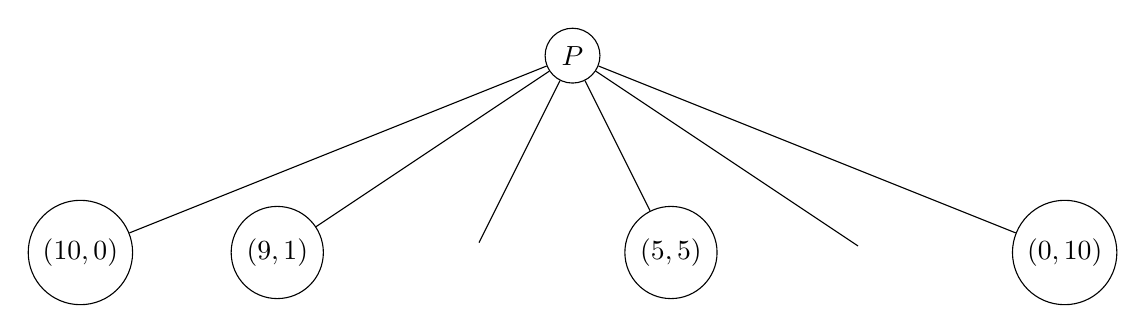
\begin{tikzpicture}[level/.style={sibling distance=25mm/#1}, level 	distance=25mm]
					\node [circle,draw] (z){$P$}
 						child {node [circle,draw] (a) {$(10, 0)$}	}
 						child {node [circle,draw] (b) {$(9, 1)$}	}
 						child {node [] (c) {$ $}	}
 						child {node [circle,draw] (d) {$(5, 5)$}	}
 						child {node [] (e) {$ $}	}
  						child {node [circle,draw] (f) {$(0, 10)$}
					};
					\path (b) -- (c) node [midway] {$\dotsc$};
					\path (c) -- (d) node [midway] {$\dotsc$};
					\path (d) -- (e) node [midway] {$\dotsc$};
					\path (e) -- (f) node [midway] {$\dotsc$};
				\end{tikzpicture}				
			\end{center}
		\item Since we have already reached the first node, a simple analyse of the reduced situation for Nash-Equilibriums returns the Sub-Game-Perfect Nash-Equilibrium. In this situation $P$ is supposed to chose $x_{p} = 10$ since it results in the highest utility value.
	\end{enumerate}
	$\Rightarrow P$ playing $x_{p} = 10$ together with R always accepting constitutes a Sub-game-Perfect Nash-Equilibrium. 

	If we look for another equilibrium it yields
		\begin{enumerate}
		\item the optimal actions
			\begin{itemize}
				\item Again, in all cases $x_{p} \in [0, 10)$ would R receive $10 - x_{p} > 0$, therefore he'd accept the offer in all cases.
				\item If he now would refuse to the offer $x_{p} = 10$ it would be plausible therefore sub-game perfect, since he indifferent between both choices.
			\end{itemize}
		\item the tree changes only slightly:
			\begin{center}
				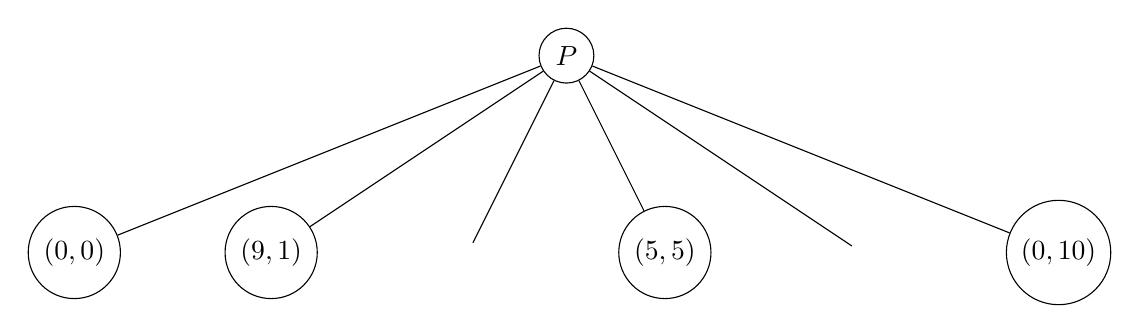
\begin{tikzpicture}[level/.style={sibling distance=25mm/#1}, level 	distance=25mm]
					\node [circle,draw] (z){$P$}
 						child {node [circle,draw] (a) {$(0, 0)$}	}
 						child {node [circle,draw] (b) {$(9, 1)$}	}
 						child {node [] (c) {$ $}	}
 						child {node [circle,draw] (d) {$(5, 5)$}	}
 						child {node [] (e) {$ $}	}
  						child {node [circle,draw] (f) {$(0, 10)$}
					};
					\path (b) -- (c) node [midway] {$\dotsc$};
					\path (c) -- (d) node [midway] {$\dotsc$};
					\path (d) -- (e) node [midway] {$\dotsc$};
					\path (e) -- (f) node [midway] {$\dotsc$};
				\end{tikzpicture}				
			\end{center}
	\end{enumerate}
	$\Rightarrow P$ playing $x_{p} = 9$ together with R always accepting if $x_{p} < 10$ and refuses for $x_{p} = 10$ also constitutes a Sub-game-Perfect Nash-Equilibrium. 
\end{example}


\begin{example}[Guessing-Game / Beauty-Contest] \index{Guessing-Game} \label{Guessing-Game}
	In a game with at least two players we can describe the sequel for a Guessing-Game (e.g. the \hyperref[Beauty-Contest]{Beauty-Contest}) as follows
	\begin{itemize}
		\item $n \geq 2$ players
		\item Every player guesses a number $b_{i} \in \{0, 1, 2, \dotsc, 100 \}$
		\item Goal is to guess $b_{i}$ as close as possible to $\frac{p}{n} \cdot \sum_{i = 1}^{n} b_{i} = p \cdot \varnothing, \quad p \in (0, 1)$
		\item The best guess (closes to $p \cdot \varnothing$) wins, in case of a tie a random device that is 'fair' decides who win the price $P > 0$
	\end{itemize}
	
	
	\textbf{1. Question:} Is $(0, \dotsc, 0)$ a Nash-Equilibrium? \\
	\textbf{Answer:} Yes. Assume all bidders except for bidder $i$ bid $0$.	
		\begin{itemize}
			\item if bidder $i$ bids $0$ expected win equals $\frac{1}{n} P $
			\item if bidder $i$ bids something above $0$ his expected profit is going to be $0$ as $0$ is closer to $p \cdot \varnothing$ then the bet $b > 0$ of player $i$:
			\[ p \cdot \varnothing = p \frac{(n - 1)0 + 1 b}{n} = p \frac{b}{n} \]
			\[
				d \left( b, p \frac{b}{n} \right) > d \left( p \frac{b}{n}, 0 \right)	\gdw \left| b - p \frac{b}{n} \right| > \left| p \frac{b}{n} \right| \quad
			\]
			
			and since $b > p \cdot \varnothing$ we can simplify this further to
			\[ b > \left( p \cdot b \right) \cdot \frac{2}{n} \quad \text{and this holds since } n \geq 2 \text{ and } p < 1.\]
		\end{itemize}
		
	
	\textbf{2. Question:} is $(0, \dotsc, 0)$ the unique Nash-Equilibrium here? \\
	\textbf{Answer:} Yes, since:	
	\[ b_{i}^{*} \leq \frac{1}{2} \frac{\sum_{j \neq i} b_{j}^{*}}{n - 1} \]
	\begin{align*}
		\Rightarrow \sum_{i = 1}^{n} b_{i}^{*} \leq \frac{1}{2} \frac{\sum_{i = 1}^{n} \sum_{j \neq i} b_{j}^{*}}{n - 1} & = \frac{1}{2} \frac{(n - 1) \sum_{j = 1}^{n} b_{j}^{*}}{n - 1} \\
		& = \frac{1}{2} \sum_{j = 1}^{n} b_{j}^{*}
	\end{align*} 
	\[ \gdw \sum_{i = 1}^{n} b_{i}^{*} \leq \frac{1}{2} \sum_{i = 1}^{n} b_{i}^{*} \]
	therefore only $(0, \dotsc,  0)$ can be a Nash-Equilibrium in this situation. \\


	\textbf{3. Question:} is $(0, \dotsc, 0)$ also a strictly dominant strategy? \\
	\textbf{Answer:} No. By analysing the following situation we find a counterexample: \\
	$50$ players. $48$ of them bid the number $100$, bidder $49$ bids $0$ then the optimal strategy for player $50$ is to bid $97$. \\
	Therefore $0$ is not the best answer and cannot be a strictly dominant strategy.
\end{example}


\newpage